\documentclass[12pt]{article}
\usepackage{sbc-template}
\usepackage{graphicx,url}
\usepackage{xspace}
\usepackage[brazil]{babel}
%\usepackage[utf8]{inputenc}
\usepackage[latin1]{inputenc}
\usepackage[T1]{fontenc}

\newcommand{\AOSD}{Projeto de Sistemas Orientados � Aplica��o}
\newcommand{\epos}{\textsc{Epos}}
\newcommand{\EPOS}{\textsc{Embedded Parallel Operating System}}
\newcommand{\aosd}{\textsc{AOSD}}
\newcommand{\tos}{\textsc{TinyOS}}
\newcommand{\framework}{\textit{framework}}
\newcommand{\ELUS}{\textsc{Elus}}
\newcommand{\elus}{\textsc{Epos Live Update System}}

\newcommand{\X}{$\bullet$}

\newcommand{\en}[1]{\emph{#1}}
\newcommand{\class}[1]{{\sffamily\bfseries{#1}}}
\newcommand{\componente}[1]{\texttt{#1}}
\newcommand{\method}[1]{\componente{#1}}
\newcommand{\proxy}{\componente{Proxy}}
\newcommand{\agent}{\componente{Agent}}
\newcommand{\handle}{\componente{Handle}}
\newcommand{\stub}{\componente{Stub}}
\newcommand{\adapter}{\componente{Adapter}}
\newcommand{\scenario}{\componente{Scenario}}
\newcommand{\msg}{\componente{Message}}
\newcommand{\vtable}{\componente{vtable}}
\newcommand{\etp}{\textsc{Elus Transport Protocol}}
\newcommand{\ETP}{\textsc{Etp}}
\newcommand{\rt}{\componente{Reconfigurator}}

\newcommand{\fig}[4][tb]{
  \begin{figure}[#1] {\centering{\includegraphics[#4]{fig/#2}}\par}
    \caption{#3\label{fig:#2}}
  \end{figure}
}

\usepackage{listings}
\lstset{keywordstyle=\bfseries, flexiblecolumns=true}
\lstloadlanguages{[ANSI]C++,HTML}
\lstdefinestyle{prg} {basicstyle=\footnotesize, lineskip=-0.2ex, showspaces=false,breaklines=true,showstringspaces=false,numbers=left,numbersep=-5pt,frame=single,stepnumber=1}

\newcommand{\prg}[3][tbp]{
  \begin{figure}[#1]
      \lstinputlisting[language=C++,style=prg]{fig/#2.cc}
    \caption{#3\label{prg:#2}}
  \end{figure}
}

\sloppy

\title{ELUS: Mecanismo de Reconfigura��o de Software para Sistemas Operacionais Embarcados}

\author{Giovani Gracioli e Ant�nio Augusto Fr�hlich}

\address{Laborat�rio de Integra��o Software e Hardware (LISHA)\\
  Universidade Federal de Santa Catarina (UFSC)\\
  Caixa Postal 476, 88049-900, Florian�polis, SC, Brasil
  \email{\{giovani,guto\}@lisha.ufsc.br}
}


\begin{document}

\maketitle

\begin{resumo}
Reconfigura��o Din�mica de Software (RDS) � o processo de atualizar o software de um sistema em execu��o. Um mecanismo de RDS para sistemas embarcados deve ser simples, transparente para aplica��es e usar o m�nimo de recursos poss�veis (e.g. mem�ria, processamento), pois estar� competindo com os recursos do pr�prio sistema embarcado.
Este artigo apresenta o \elus{} (\ELUS{}), uma infra-estrutura de sistema operacional que permite reconfigura��o din�mica de software em sistemas embarcados. \ELUS{} faz uso de sofisticadas t�cnicas de metaprograma��o est�tica em C++, consumindo pouca mem�ria e tornando o processo de reconfigura��o configur�vel, simples e totalmente transparente para as aplica��es.
\end{resumo}

\begin{abstract}
Dynamic software reconfiguration is the process of updating the system software during its execution. A dynamic software reconfiguration mechanism for an embedded system must be simple, transparent to applications, and use the minimum amount of resources (e.g. memory, processing) possible, since it shares resources with the target embedded system. We present \elus{} (\ELUS{}), an operating system infrastructure for resource-constrained embedded systems. Through the use of sophisticated C++ static metaprogramming techniques, unlike the previous software reconfiguration infrastructures, \ELUS{} provides a low-overhead, simple,
configurable, and fully transparent software reconfiguration mechanism. %Our experimental evaluation shows that the \ELUS{} memory consumption, overhead, and reconfiguration time present better performance when compared to related work.
\end{abstract}

% 1 - Introduction
\section{Introdu��o}

Reconfigura��o Din�mica de Software (RDS) � uma caracter�stica presente na grande maioria dos sistemas atuais, desde ambientes de computa��o convencionais (e.g. computadores pessoais) at� sistemas embarcados (e.g. sensores sem fio). Com a finalidade de corrigir bugs, adicionar e/ou remover funcionalidades e adaptar o sistema �s variabilidades dos ambientes de execu��o, esta caracter�stica permite que o software do sistema seja atualizado em tempo de execu��o.

Redes de Sensores Sem Fio (RSSF), por exemplo, podem ser formadas por um grande n�mero de sensores espalhados em um ambiente de monitora��o. Geralmente, estes sensores possuem poucos kilobytes de mem�ria e poder de processamento~\cite{asada98wireless}. Frequentemente, coletar todos os sensores para reprograma��o � impratic�vel devido � grande quantidade ou ao dif�cil acesso �s �reas de monitora��o. Para estes casos, um mecanismo eficiente de RDS poderia reprogramar todos os nodos da rede remotamente. Al�m disso, o mecanismo de RDS tamb�m deve ser adapt�vel a grande variabilidade de plataformas de sistemas embarcados existentes em termos de recursos de mem�ria, interconex�es (e.g. RS-485, CAN, ZigBee) e poder de processamento.

N�o obstante, a infra-estrutura de reconfigura��o din�mica de software para sistemas embarcados compartilha recursos com as aplica��es do sistema e n�o deve influenciar sua opera��o~\cite{update}. Mecanismos para RDS em sistemas embarcados podem ser divididos em tr�s categorias: (i) atualiza��o de c�digo bin�rio~\cite{reijers03efficient, flexcup, update}; (ii) m�quinas virtuais~\cite{mate, Koshy2005, Xie2006}; e (iii) sistemas operacionais~\cite{dunkels04contiki, sos, Cha2007, Bagchi2008}. Na primeira, um bootloader ou ligador � respons�vel por receber e atualizar a nova imagem do sistema. Na segunda, a reconfigura��o � realizada atrav�s da atualiza��o do script da aplica��o que � interpretado pela m�quina virtual. Finalmente, sistemas operacionais s�o projetados para abstrair uma atualiza��o de software. Tais SOs s�o organizados em m�dulos reconfigur�veis e criam um n�vel de indire��o entre a aplica��o que utiliza o m�dulo e o m�dulo propriamente dito atrav�s de ponteiros e/ou tabelas. A reconfigura��o neste caso ocorre mudando o endere�o desses m�dulos dentro das tabelas/ponteiros.

Este artigo apresenta o \elus{} (\ELUS{}), uma infra-estrutura de SO para sistemas embarcados com recursos limitados. O \ELUS{} � constru�do dentro do framework de componentes do \EPOS{} (\epos{}), em torno do programa de aspecto de invoca��o remota de m�todos~\cite{Froehlich:2001}. As principais caracter�sticas que tornam o \ELUS{} diferente das infra-estruturas de SO existes s�o:

\begin{itemize}
 \item \textbf{Configurabilidade:} componentes do sistema\footnote{Componentes no \epos{} s�o encapsulados em classes C++ com interface e comportamento bem definidos.} podem ser marcados como reconfigur�veis ou n�o em tempo de compila��o. Para todos os componentes n�o-reconfigur�veis, nenhum sobrecusto em termos de processamento e mem�ria � adicionado ao sistema.

 \item \textbf{Baixo Consumo de Mem�ria:} ao marcar um componente como reconfigur�vel, s�o adicionados cerca de 1.6KB de mem�ria e 26 bytes de dados por componente, o que presenta um baixo consumo comparado com os trabalhos relacionados.

 \item \textbf{Transpar�ncia e Simplicidade:} uma reconfigura��o � realizada atrav�s de um simples protocolo, o \etp{} (\ETP{}). Al�m disso, tanto a infra-estrutura de reconfigura��o como a reconfigura��o de software s�o totalmente transparentes para as aplica��es.

 \item \textbf{Estrutura de Mensagens:} atrav�s do uso da estrutura do framework do \epos{}, a passagem de argumentos e valor de retorno entre os componentes do sistema � realizada eficientemente, cerca de 5 vezes mais r�pida do que os trabalhos anteriores.

 \item \textbf{Reconfigura��o:} \ELUS{} permite que o desenvolvedor atualize ambos componentes do SO e aplica��es. Em alguns SOs, como Contiki~\cite{dunkels04contiki} por exemplo, somente aplica��es ou partes do SO s�o reconfigur�veis.
\end{itemize}

O restante deste artigo est� organizado da seguinte maneira: a se��o~\ref{sec:epos} apresenta o framework metaprogramado do \epos{}. A se��o~\ref{sec:elus} explica o projeto e a implementa��o do \ELUS{}. A avalia��o experimental � relatada na se��o~\ref{sec:evaluation}. A se��o~\ref{sec:rel} apresenta os trabalhos relacionados.
A se��o~\ref{sec:analysis} compara os trabalhos relacionados com o \ELUS{}. Finalmente, a se��o~\ref{sec:conc} conclui o artigo.


\section{Framework Metaprogramado do \epos{}}
\label{sec:epos}

%\epos{} � um SO para sistemas embarcados multi-plataforma baseado em componentes~\cite{Froehlich:2001}. \epos{} tem um arquitetura altamente escal�vel que � moldada para suportar as necessidades das aplica��es. \epos{} implementa aspectos atrav�s de adaptadores de cen�rios~\cite{Froehlich:sci:2000}. Combina��es distintas de componentes do sistema e adaptadores de cen�rios acarreta a diferentes arquiteturas de software. Neste contexto, \epos{} implementa um framework que define como os componentes s�o organizados em um sistema funcional. O framework � realizado por um metaprograma est�tico em C++, sendo assim executado na compila��o do sistema, adaptando os componentes selecionados para coexistir entre eles e as aplica��es.

\epos{} � um SO para sistemas embarcados multi-plataforma baseado em componentes que possui uma arquitetura altamente escal�vel moldada para suportar as necessidades das aplica��es~\cite{Froehlich:2001}. O \epos{} implementa aspectos\footnote{Como na tradicional programa��o orientada a aspectos (AOP).} atrav�s de adaptadores de cen�rios~\cite{Froehlich:sci:2000}, que quando combinados com distintos componentes do sistema, formam diferentes arquiteturas de software. Neste contexto, o \epos{} implementa um framework que define como os componentes s�o organizados de forma a gerar um sistema funcional. O framework � realizado por um metaprograma est�tico em C++, sendo assim executado na compila��o do sistema, adaptando os componentes selecionados para coexistir entre eles, aspectos e as aplica��es.

\begin{figure}
 \hspace{0.033\textwidth}
 \begin{minipage}{0.45\textwidth}
  \centering
  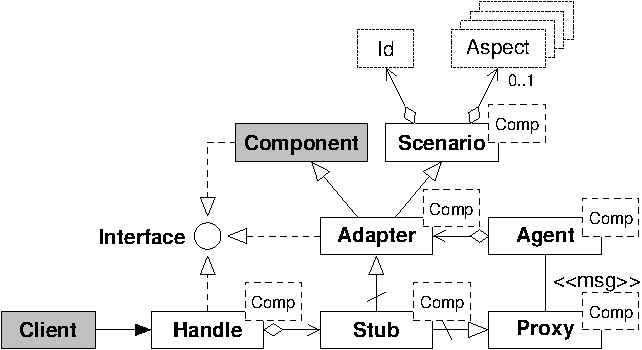
\includegraphics[scale=0.5]{fig/framework}
  \caption{Framework metaprogramado do \epos{}.}
  \label{fig:framework}
  \end{minipage}
  \begin{minipage}{0.45\textwidth}
  \centering
  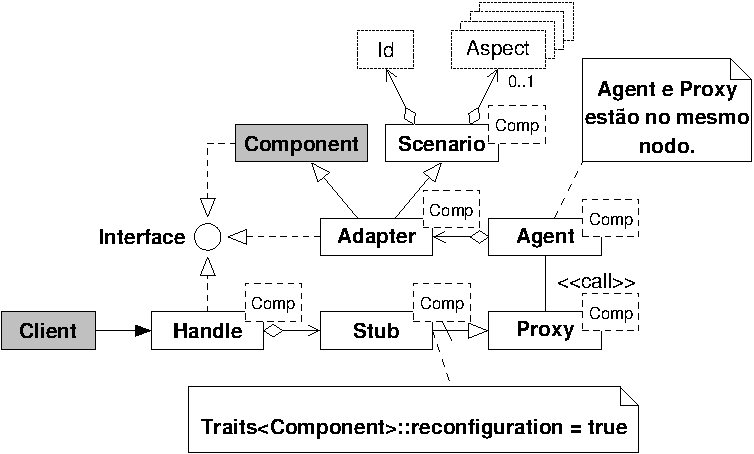
\includegraphics[scale=0.5]{fig/epos_fmk_reconf}
  \caption{Framework para RDS.}
  \label{fig:framework-reconf}
  \end{minipage}
\end{figure}

% \begin{figure}
% \centering
% \begin{tabular}{c c}
% 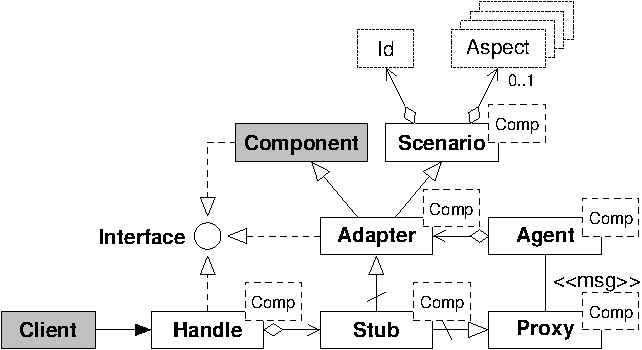
\includegraphics[scale=0.5]{fig/framework} & 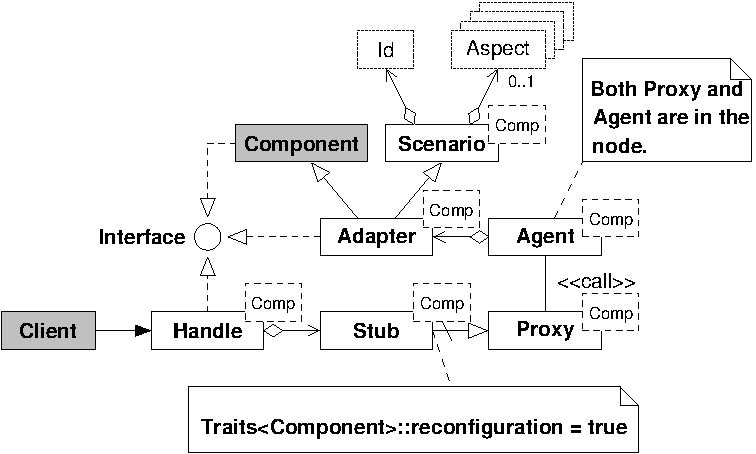
\includegraphics[scale=0.5]{fig/framework-reconf} \\
% (a) Framework metaprogramado do \epos{}. & (b) Framework para reconfigura��o. \\
% \end{tabular}
% \caption{(a) Vis�o geral do framework metaprogramado do \epos{}~\cite{Froehlich:2001}. (b) Framework metaprograma do \epos{} para reconfigura��o de software.}
% \label{fig:framework}
% \end{figure}

Uma vis�o geral do framework metaprogramado do \epos{} � demonstrado na Figura~\ref{fig:framework}. Um cliente (aplica��o ou componente) deseja invocar um m�todo de um componente (e.g. Thread, UART, etc). A classe parametrizada \handle{} recebe um componente do sistema como par�metro. Ela verifica se o objeto foi corretamente criado e encaminha a invoca��o de m�todo ao elemento \stub{} que verifica se o aspecto de invoca��o remota est� ativo para o componente (o aspecto � selecionado pelo componente atrav�s de sua classe \textit{Trait}~\cite{Stroustrup:1997}). Se o aspecto n�o est� habilitado, \stub{} herdar� o adaptador de cen�rio do componente, caso contr�rio herdar� o \proxy{} do componente (\textit{Stub$<$Componente, true$>$}). Consequentemente, se \textit{Traits$<$Componente$>$::remote = false} ent�o \handle{} usa o adaptador de cen�rio como \stub{}; se verdadeiro, \handle{} usa o \proxy{}.

O elemento \proxy{} � respons�vel por enviar uma mensagem com a invoca��o do m�todo do componente para o seu \agent{}. A mensagem cont�m os identificadores do objeto, m�todo e classe que s�o usados pelo \agent{} para invocar o m�todo correto, associando-os a uma tabela de m�todos. O elemento \agent{} recebe esta mensagem e invoca o m�todo atrav�s do \adapter{}. A classe \adapter{} aplica os aspectos suportados pelo \scenario{} antes e depois da chamada real do m�todo. Cada inst�ncia do \scenario{} consulta o \textit{Traits} do componente para verificar quais aspectos est�o habilitados, agregando o aspecto de cen�rio correspondente. Quando um aspecto n�o � selecionado para o componente, uma implementa��o vazia � utilizada. Neste caso, nenhum c�digo � gerado na imagem final do sistema, similar a um \textit{aspect weaver} na programa��o orientada a aspectos tradicional. 

A estrutura do framework � totalmente transparente para as aplica��es devido ao uso de dois \textit{namespaces}: um para as aplica��es e outro para o sistema. Em tempo de compila��o, os componentes do sistema s�o exportados para o \textit{namespace} da aplica��o, conforme demonstra a Figura~\ref{prg:export}. Consequentemente, uma invoca��o de m�todo da aplica��o para um componente do sistema � realizada da mesma maneira, mas ao inv�s de chamar o m�todo real, a chamada � feita atrav�s do framework. Da mesma foram, quando componentes do sistema desejam invocar m�todos de componentes reconfigur�veis tamb�m devem faz�-lo atrav�s do \textit{namespace} da aplica��o.

\prg{export}{Exportando um componente para o \textit{namespace} da aplica��o.}

Foi observado neste trabalho que a estrutura \proxy{}/\agent{} do framework cria um n�vel de indire��o entre as invoca��es de m�todos do cliente para os componentes do sistema que possuem o aspecto de invoca��o remota habilitado, isolando os componentes e os tornando independente de posi��o na mem�ria. Neste cen�rio, da perspectiva do cliente, uma invoca��o remota � realizada sem o conhecimento da localiza��o do componente. Essa isola��o pode tamb�m ser aplicada para RDS, pois somente o \agent{} � ciente da posi��o do componente na mem�ria. Diferentemente do aspecto de invoca��o remota presente no \epos{}, este trabalho prop�e substituir a invoca��o de m�todo entre o \proxy{} e \agent{} para uma simples invoca��o de m�todo entre eles. Sendo assim, o mesmo n�vel de indire��o pode residir no mesmo espa�o de endere�amento de um nodo. A Figura~\ref{fig:framework-reconf} exemplifica este cen�rio na estrutura do framework.


\section{\elus{}}
\label{sec:elus}

Para que uma reconfigura��o de software seja executada de maneira segura e sem comprometer o sistema como um todo, existem tr�s \textbf{requisitos principais} que devem ser satisfeitos~\cite{Polakovic2008}:

\begin{itemize}
 \item \textbf{Estado quiescente}: para que uma reconfigura��o possa acontecer corretamente, o sistema deve atingir um estado de execu��o considerado consistente, pass�vel de reconfigura��o, chamado de estado quiescente~\cite{bloom1993, soules03system}. Em um ambiente com m�ltiplas threads, como o \epos{}, o estado quiescente de um componente � atingido quando nenhuma das threads est� invocando m�todos deste componente~\cite{Polakovic2008}.

 \item \textbf{Transfer�ncia de estado}: ap�s o sistema atingir o estado quiescente, o estado (dados) do componente antigo deve ser transferido para o novo componente, se necess�rio. Isto pode ser realizado atrav�s da c�pia dos dados privados do antigo componente para o novo, atrav�s da cria��o de um novo objeto passando os dados do objeto antigo para o construtor do componente e deletando o objeto antigo ou ainda atrav�s dos m�todos \method{set} e \method{get}~\cite{Polakovic2008}.

 \item \textbf{Ajuste das refer�ncias}: ap�s a transfer�ncia de estado, as refer�ncias que o sistema utilizava para acessar o antigo c�digo do componente devem ser atualizadas para apontarem para o novo c�digo, de forma que a aplica��o continue sua execu��o invocando os m�todos corretamente.
\end{itemize}

Adicionalmente a esses requisitos, sistemas embarcados ainda apresentam s�rias limita��es em termos de mem�ria e, quando s�o alimentados por bateria, deve-se respeitar limita��es no consumo de energia. Por esta raz�o, o pr�prio sistema de reconfigura��o deve utilizar o m�nimo de recursos poss�veis, pois estar� compartilhando recursos com a(s) aplica��o(�es). Reduzir o n�mero de transfer�ncia de dados pela rede e o n�mero de escritas/leituras na mem�ria do sistema s�o \textbf{requisitos desej�veis} para que o sistema consiga realizar as suas atividades por um maior per�odo de tempo. Da mesma forma, reduzir a quantidade de mem�ria utilizada pelo mecanismo de reconfigura��o resultar� em maior espa�o de mem�ria livre para a aplica��o.

\subsection{Premissas}

Em fun��o dos requisitos apresentados na se��o anterior, o projeto do \ELUS{} baseou-se nas seguintes premissas:

\begin{itemize}
  \item A unidade de reconfigura��o do sistema � componente. Os componentes s�o classes que devem ser implementados na linguagem C++ e poder�o ser marcados como reconfigur�veis ou n�o em tempo de compila��o. Para aqueles componentes n�o reconfigur�veis nenhum sobrecusto dever� ser adicionado ao sistema. Somente os componentes que possuem reconfigura��o habilitada no sistema s�o pass�veis de atualiza��o.

  \item O estado quiescente do componente que est� sendo reconfigurado dever� ser alcan�ado antes da sua reconfigura��o. Desta forma, a reconfigura��o de software ser� realizada de forma consistente e n�o comprometer� as atividades realizadas pela aplica��o.

  \item N�o s�o permitidas mudan�as na API do sistema. As assinaturas dos m�todos dos componentes devem permanecer as mesmas em ambas vers�es. Esta caracter�stica restringe o escopo de reconfigura��o, mas por outro lado, devido a resolu��o das depend�ncias entre os componentes e a aplica��o e pelas otimiza��es realizadas pelo compilador na compila��o do sistema, o c�digo gerado apresentar� um bom desempenho.

  \item O hardware do sistema n�o sofre mudan�as. Tanto a vers�o que est� sendo reconfigurada quanto a vers�o antiga executam sobre a mesma plataforma.

  \item � tarefa do desenvolvedor garantir que o novo componente n�o remova nenhum m�todo que est� sendo utilizado por outros componentes. O \ELUS{} n�o ser� respons�vel por verificar depend�ncias de chamadas de m�todos entre componentes do sistema.

  \item Os m�todos reconfigur�veis do componente dever�o ter sido declarados como virtuais. Ao declarar um m�todo como virtual, o compilador ir� gerar uma tabela de m�todos virtuais (\vtable{}) que cont�m os endere�os dos m�todos do componente. A \vtable{} ser� utilizada para ajustar as refer�ncias para os m�todos ap�s uma reconfigura��o.

  \item Os atributos de um componente reconfigur�vel dever�o ser acessados exclusivamente atrav�s dos m�todos \componente{set} e \componente{get} relacionados ao atributo.
\end{itemize}

\subsection{Arquitetura}

A arquitetura do \ELUS{} � apresentada na Figura~\ref{fig:architecture_v2_pt.pdf}. O framework original foi estendido para suportar reconfigura��o de software. O elemento \agent{} � o �nico ciente da posi��o dos componentes em mem�ria. Este elemento possui uma ``OS Box'' que armazena as mensagens enviadas pelo \proxy{} e controle o acesso aos m�todos do componente atrav�s de um sincronizador (Sem�foro) para cada componente, evitando que um m�todo de um componente que esteja sendo reconfigurado seja chamado ao mesmo tempo. Essa ``Box'' tamb�m funciona como um ponto de acesso, chamando os m�todos do componente no \agent{} atrav�s de uma tabela de m�todos. O \agent{} encaminha a chamada ao \adapter{} que invoca os m�todos do componente atrav�s da \vtable{} do objeto, ap�s recuper�-lo em uma tabela hash.

\fig{architecture_v2_pt.pdf}{Arquitetura do \ELUS{}.}{scale=0.6}

%\fig{architecture_v2.pdf}{Arquitetura do \ELUS{}.}{totalheight=0.18\textheight, width=0.48\textwidth}

O framework � um metaprograma, no qual todas as suas depend�ncias entre um componente e os cen�rios de execu��es s�o resolvidas durante a compila��o do sistema. Portanto, o \proxy{} � dissolvido no c�digo do cliente pelo compilador. Desta forma, chamadas do \proxy{} ao \agent{} s�o realizadas diretamente do cliente para a ``OS Box''. No c�digo final gerado, os elementos \proxy{}, \handle{} e \stub{} n�o existem.

A Figura~\ref{fig:proxy_agent.pdf} mostra os novos elementos \proxy{} e \agent{} do framework do \ELUS{}. Eles s� estar�o presentes se a reconfigura��o estiver habilitada para um componente. A classe \proxy{} realiza os m�todos do componente e usa a classe \msg{} para encaminhar uma invoca��o de m�todo ao \agent{}. Quando o \proxy{} recebe um pedido do \handle{}, ele preenche a mensagem com os IDs do m�todo e componente e com os par�metros do m�todo. A classe \msg{} possui uma interface para anexar e recuperar par�metros e valor de retorno (m�todos \textit{in} e \textit{out}). O m�todo \textit{invoke} da classe chama a fun��o \textsc{OS Box}, na qual usa um vetor (\textit{Dispatcher}) para entregar as chamadas ao \agent{}. O \agent{}, por sua vez, reconfigura o componente atrav�s de uma chamada ao m�todo \textbf{update} que utiliza um gerenciador de c�digo para realizar escritas e leituras na mem�ria de programa. Uma Thread, chamada de \textsc{Reconfigurator}, criada na inicializa��o do sistema, recebe um pedido de reconfigura��o e o novo c�digo do componente por uma interface de rede (RS-232 ou r�dio por exemplo). Esse pedido � enviado para o \agent{} atrav�s da ``OS Box'' em uma mensagem usando um formato espec�fico, chamado de \etp{} (\ETP{}). Um novo componente ao ser atualizado � compilado e ligado com a imagem gerada do sistema e seu c�digo enviado pela rede. Este novo c�digo do componente � ligado usando o endere�o da fun��o \textsc{OS Box}, na qual � o ponto de entrada para a estrutura do framework. Consequentemente, esta fun��o � o �nico elemento do sistema que \textbf{n�o �} reconfigur�vel.

%\figspan{proxy_agent.pdf}{\ELUS{} Proxy and Agent elements.}{scale=.5}
%\fig{proxy_agent.pdf}{\ELUS{} Proxy and Agent elements.}{totalheight=0.2\textheight, width=0.48\textwidth}

O \ETP{} define 6 tipos de mensagens de reconfigura��o: (a) adi��o de m�todo em um componente; (b) remo��o de m�todo de um componente; (c) atualiza��o de um componente; (d) atualiza��o de um endere�o de mem�ria espec�fico; (e) atualiza��o da aplica��o; e (f) adi��o de atributo. As Figuras~\ref{fig:msg_upd} e ~\ref{fig:msg_app} exemplificam as mensagens de atualiza��o de componente e aplica��o. O campo de controle identifica qual o tipo da mensagem. Um componente especial (\textit{Application Update}) foi criado para atualizar a aplica��o e reiniciar o sistema ap�s a sua atualiza��o.

% \begin{figure}
%   \hspace{0.0\textwidth}
%   \begin{minipage}{0.3\textwidth}
%    \centering
%    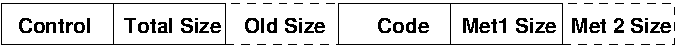
\includegraphics[scale=0.38]{fig/msg_upd_en}
%    \caption{Mensagem de atualiza��o de componente.}
%    \label{fig:msg_upd}
%    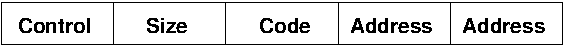
\includegraphics[scale=0.4]{fig/msg_app_en}
%    \caption{Mensagem de atualiza��o de aplica��o.}
%    \label{fig:msg_app}
%  \end{minipage}
%  \hspace{0.08\textwidth}
%   \begin{minipage}{0.6\textwidth}
%    \centering
%  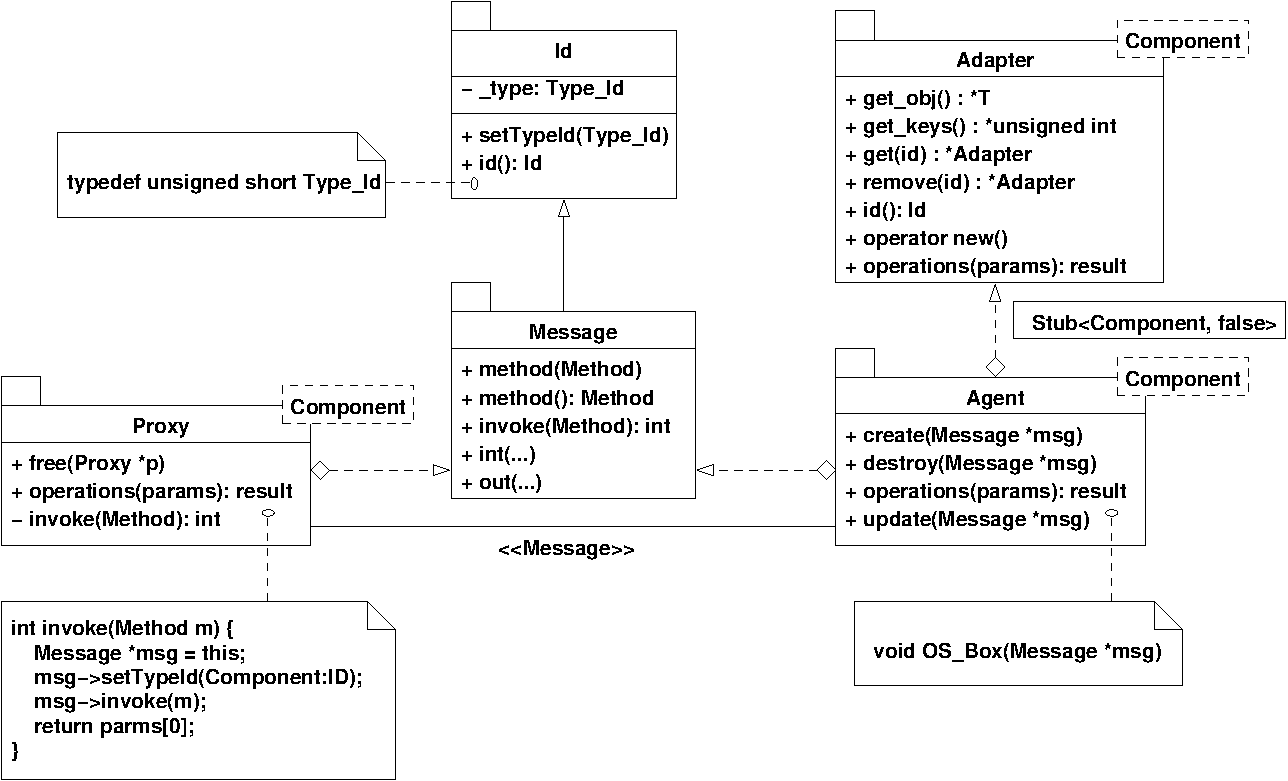
\includegraphics[totalheight=0.2\textheight, width=\textwidth]{fig/proxy_agent}
%  \caption{Elementos \proxy{}, \agent{}, \adapter{} e \msg{} do framework do \ELUS{}.}
%  \label{fig:proxy_agent.pdf}
%  \end{minipage}
%  \end{figure}

\begin{figure}
 \hspace{0.0\textwidth}
  \begin{minipage}{0.6\textwidth}
   \centering
 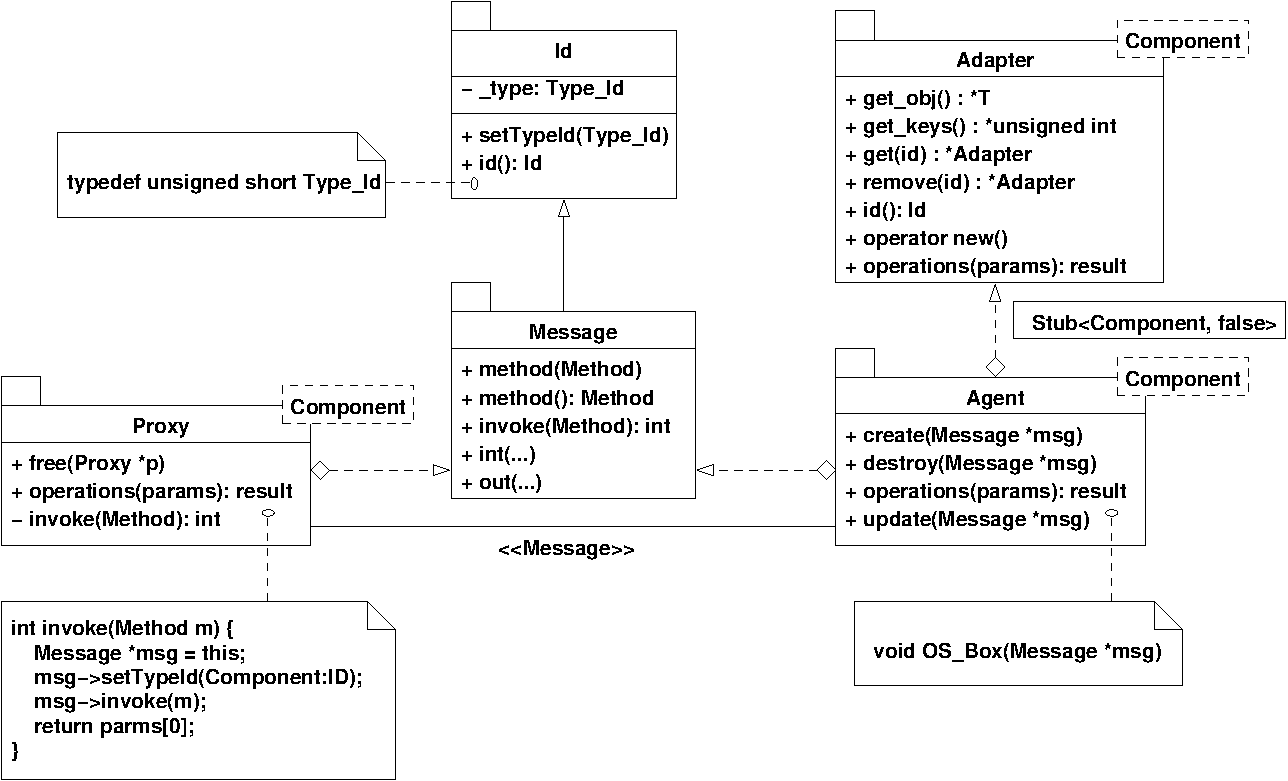
\includegraphics[totalheight=0.2\textheight, width=\textwidth]{fig/proxy_agent}
 \caption{Elementos \proxy{}, \agent{}, \adapter{} e \msg{} do framework do \ELUS{}.}
 \label{fig:proxy_agent.pdf}
 \end{minipage}
\hspace{0.0\textwidth}
  \begin{minipage}{0.3\textwidth}
   \centering
   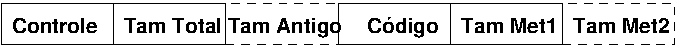
\includegraphics[scale=0.38]{fig/msg_upd_pt}
   \caption{Mensagem de atualiza��o de componente.}
   \label{fig:msg_upd}
   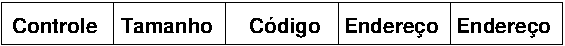
\includegraphics[scale=0.4]{fig/msg_app_pt}
   \caption{Mensagem de atualiza��o de aplica��o.}
   \label{fig:msg_app}
 \end{minipage}

 \end{figure}


%\fig{updateAgent.pdf}{Sequence diagram of the Agent update method when performing a component updating.}{totalheight=0.35\textheight, width=0.7\textwidth}



\section{Avalia��o}
\label{sec:evaluation}

A avalia��o do \ELUS{} considerou tr�s m�tricas: consumo de mem�ria, sobrecusto nas chamadas de m�todos introduzido pelo n�vel de indire��o e \vtable{} e tempo de reconfigura��o. Foi usado o compilador GNU g++ 4.0.2 e a ferramenta GNU \textit{objdump} 2.16.1 para gerar o sistema e analisar as m�tricas. A plataforma utilizada na avalia��o foi o Mica2, composto de um microcontrolador ATMega128, com 4KB de RAM, 128KB de Flash, 4KB de EEPROM e um conjunto de perif�ricos incluindo comunica��o via r�dio.

\subsection{Consumo de Mem�ria}

Na primeira avalia��o, o suporte � RDS foi habilitado somente para o componente \textit{Chronometer} composto por 8 m�todos atualiz�veis~\cite{timer}. O objetivo foi medir o sobrecusto de mem�ria associado � infra-estrutura do framework. A Tabela~\ref{tab:memory} apresenta o consumo de mem�ria dos elementos do \ELUS{}. O framework necessitou de cerca de 2.6KB de mem�ria de c�digo, 42 bytes de dados para o \textit{Dispatcher} e atributos de controle e 52 bytes para dados n�o-inicializados para tabela hash. \textsc{Reconfigurator} precisou de 70 bytes de dados para o buffer de recebimento de dados via rede (40 bytes) e vari�veis de controle. \textsc{Application Update} usou 210 bytes de mem�ria de c�digo. Para esta configura��o, o total de mem�ria utilizada foi 3.5KB de c�digo e 148 bytes de dados.

\begin{table}
 \hspace{0.0\textwidth}
 \begin{minipage}{0.48\textwidth}
  \centering
\scriptsize{
\caption{Consumo de mem�ria do \ELUS{}.} 
\begin{tabular}{|c|c|c|c|c|}\hline
\textbf{\ELUS{}} & \multicolumn{4}{c|}{\textbf{Tamanho Se��o (bytes)}} \cr
\cline{2-5}
\textbf{Elementos} & \textbf{.text} & \textbf{.data} & \textbf{.bss} & \textbf{.bootloader} \cr
\hline
\textbf{Reconfigurator} 	& 410 & 0 & 70 & 0  \cr\hline
\textbf{Code Manager} 		& 16 & 0 & 2 & 375  \cr\hline
\textbf{App. Update} 		& 210 & 0 & 0 & 0  \cr\hline
\textbf{OS Box} 		& 76 & 0 & 0 & 0  \cr\hline
\textbf{Framework} 		& 2620 & 43 & 52 & 0  \cr\hline
\hline
\textbf{Total} & 3452 & 43 & 124 & 375 \cr
\hline
\end{tabular}
}
\label{tab:memory}
\end{minipage}
 \hspace{0.0\textwidth}
 \begin{minipage}{0.48\textwidth}
  \centering
\scriptsize{
\caption{Tempo de reconfigura��o para um componente.}
\begin{tabular}{c|c|c|}
\cline{2-3}
 & \multicolumn{2}{|c|}{\textbf{Tempo (em ciclos)}}\cr
\cline{2-3}
 & \textbf{Atualiza��o} & \textbf{Atualiza��o} \cr
& \textbf{mesma posi��o} & \textbf{nova posi��o} \cr
\cline{1-3}
\multicolumn{1}{|c|}{\textbf{Agent Update}} & 238 & 290 \cr
\hline
\multicolumn{1}{|c|}{\textbf{Reconfigurator}}  & 65 & 65 \cr
\hline
\multicolumn{1}{|c|}{\textbf{OS Box}} & 59 & 59 \cr
\hline
\hline
\multicolumn{1}{|c|}{\textbf{Total}}	& 362 & 414 \cr\hline
\end{tabular}
}
\label{tab:time}
\end{minipage}
\end{table}

O segundo teste de mem�ria avaliou o consumo dos m�todos individuais do framework para um componente gen�rico. Este teste considerou somente o consumo de mem�ria do framework, desprezando a mem�ria necess�ria pelo componente. O objetivo foi medir o sobrecusto adicionado quando um componente � marcado como reconfigur�vel. A Figura~8 apresenta os valores dessa avalia��o. O total m�nimo com o construtor, destrutor, o m�todo de atualiza��o e um m�todo sem par�metro e valor de retorno para um componente foi de 1.6KB de c�digo e 26 bytes de dados.

\begin{figure}
 \hspace{0.0\textwidth}
 \begin{minipage}{0.48\textwidth}
  \centering
\scriptsize{
\caption{Consumo de mem�ria dos m�todos individuais do framework do \ELUS.}
\begin{tabular}{|c|c|c|}\hline
\textbf{M�todo} & \multicolumn{2}{c|}{\textbf{Tamanho da se��o (bytes)}} \cr
\cline{2-3}
\textbf{do Framework} & \textbf{.text} & \textbf{.data} \cr
\hline
Create				& 180  & 0  \cr\hline
Destory 			& 138  & 0  \cr\hline
M�todo sem par�metro  	& 94 & 0  \cr
e valor de retorno 		& & 	\cr\hline
M�todo com um par�metro   	& 98 & 0  \cr
e sem valor de retorno 	& &  \cr\hline
M�todo sem par�metro 	& 112  & 0  \cr
e com valor de retorno 		& &  \cr\hline
M�todo com um par�metro  	& 126 & 0  \cr
e valor de retorno 		& &  \cr\hline
Update	 			& 1250  & 0   \cr\hline
Dispatcher 			& 0  & 2 X (n. de m�todos)  \cr\hline
Semaphore 			& 0  & 18   \cr\hline
\hline
\textbf{Tamanho m�nimo}  & 1662 & 26 \cr
\hline
\end{tabular}
}
\label{tab:per}
\end{minipage}
\hspace{0.0\textwidth}
 \begin{minipage}{0.48\textwidth}
  \centering
  %\fig{invTime.pdf}{Comparison of invocation time among a regular method invocation, through vtable and through \ELUS{}.}{totalheight=0.2\textheight, width=0.45\textwidth}
  \caption{Compara��o dos tempos de invoca��o de m�todo entre uma invoca��o normal, atrav�s da vtable e do \ELUS{}.}
  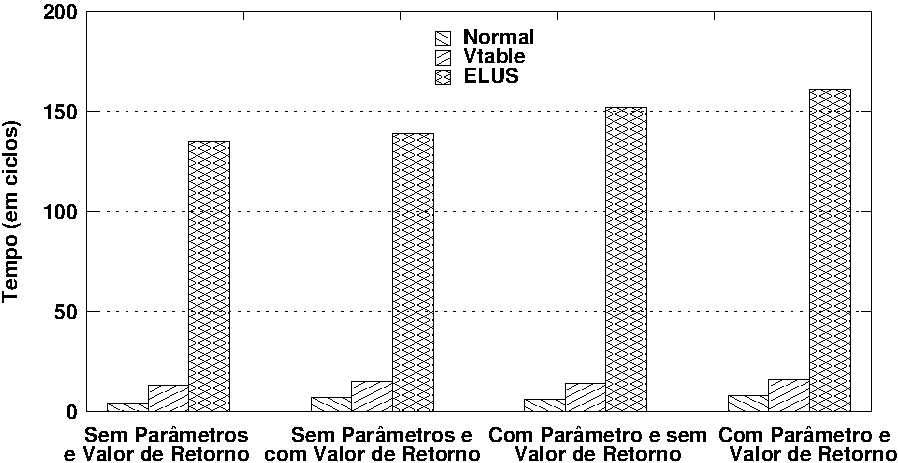
\includegraphics[totalheight=0.235\textheight, width=\textwidth]{fig/invTime_pt}
  \label{fig:invTime}
\end{minipage}
\end{figure}


\subsection{Tempo de Invoca��o de M�todo}

O n�vel de indire��o entre uma aplica��o e um componente cria um sobrecusto de invoca��o. Antes da chamada real do m�todo, o \agent{} deve recuperar os argumentos da mensagem, o objeto associado ao componente em uma tabela hash e finalmente chamar o m�todo atrav�s da sua \vtable{}. A Figura~\ref{fig:invTime} apresenta uma compara��o entre os tempos de invoca��o de m�todos de um componente normal, atrav�s de uma \vtable{} e atrav�s do \ELUS{}, usando 4 tipos de m�todos. O desempenho do \ELUS{} foi cerca de 10 vezes pior que a \vtable{}. Como ser� visto na Se��o~\ref{sec:analysis}, esse desempenho � melhor que os trabalhos relacionados.

\subsection{Tempo de Reconfigura��o}

A Tabela~2 apresenta os tempos de reconfigura��o em 2 cen�rios de atualiza��o: (i) quando o novo c�digo de um componente � menor ou igual ao antigo, sendo assim uma atualiza��o na mesma posi��o do componente e (ii) quando o novo c�digo de um componente � maior que o antigo, identificando uma atualiza��o em uma nova posi��o. Por motivos de compara��o com os trabalhos relacionados, este teste n�o considerou o tempo de recebimento de dados pela rede no \textsc{Reconfigurator} e o tempo de escrita dos dados na flash. Foram considerados os tempos de chamada do \textsc{Reconfigurator} para a ``SO Box'', o tempo na ``SO Box'' para acessar o \textit{Dispatcher} e chamar o m�todo \textit{update} do \agent{} e o tempo para o \agent{} recuperar os dados e executar uma reconfigura��o.

O \textsc{Reconfigurator} consome 65 ciclos do microcontrolador para chamar a ``SO Box''. A ``SO Box'' consome 59 ciclos para atingir o estado quiescente (opera��es \textit{p()} e \textit{v()} no sem�foro) e chamar o m�todo \textit{update} do \agent{}. Finalmente, o m�todo de atualiza��o gasta 238 ciclos para executar uma atualiza��o no cen�rio (i) e 290 ciclos no cen�rio (ii).


\section{Trabalhos Relacionados}
\label{sec:rel}

\textsc{TinyOS} � considerado o SO mais popular para RSSF. � um SO orientado a eventos e originalmente n�o suporta reconfigura��o de software~\cite{hill00system}. Entretanto, diversos trabalhos t�m sido realizados com o intuito de suportar reconfigura��o no \textsc{TinyOS}~\cite{mate, deluge, flexcup}. \textsc{MantisOS} � outro SO para RSSF muito conhecimento no ambiente acad�mico, mas n�o suporta reconfigura��o~\cite{mantis}.

\textsc{Nano-Kernel} permite RDS das aplica��es e dos componentes do kernel atrav�s da separa��o dos dados e dos algoritmos l�gicos do kernel~\cite{Bagchi2008}. � criado um n�vel de indire��o entre as aplica��es e os dispositvos do kernel (e.g. escalonador, gerenciador de mem�ria, etc). O n�cleo do \textsc{Nano-Kernel} e os dispositivos do kernel se comunicam atrav�s de interfaces espec�ficas que devem ser iniciadas na inicializa��o do sistema.

\textsc{RETOS} implementa RDS atrav�s de reloca��o din�mica de mem�ria e liga��o em tempo de execu��o~\cite{Cha2007}. O processo de reloca��o extrai informa��es de vari�veis e fun��es globais em tempo de compila��o (meta-informa��es) que s�o colocadas em um arquivo no formato \textsc{RETOS}. Tais informa��es s�o utilizadas pelo kernel para substituir todo endere�o acess�vel de um m�dulo quando o estiver carregando. O SO possui uma tabela com endere�os para fun��es de outros m�dulos. Um m�dulo registra, desregistra e acessa fun��es atrav�s desta tabela.

\textsc{Contiki} � um SO para RSSF que implementa processos especiais, chamados de \emph{servi�os}, que prov�em funcionalidades a outros processos~\cite{dunkels04contiki}. Servi�os s�o substitu�dos em tempo de execu��o atrav�s de uma \emph{interface stub} respons�vel por redirecionar as chamadas das fun��es para uma \emph{interface de servi�o}, que possui ponteiros para as implementa��es atuais das fun��es do servi�o correspondente. \textsc{Contiki} somente permite a atualiza��o de algumas partes do sistema.

\textsc{SOS} � um SO para RSSF que permite RDS~\cite{sos}. O SO � constru�do em m�dulos que s�o inseridos, removidos ou substitu�dos em tempo de execu��o. Atrav�s do uso de chamadas relativas, o c�digo em cada m�dulo torna-se independente de posi��o da mem�ria. 

\ELUS{} � conceitualmente similar aos trabalhos relacionados apresentados, por�m a infra-estrutura do framework possui a vantagem de eliminar parte do sobrecusto associado �s tabelas de indire��o com o uso da metaprograma��o est�tica. Tabela~\ref{tab:reconf2} revisa o processo de reconfigura��o nos SO embarcados analisados.

\begin{table}[ht]
\centering
\caption{Caracter�sticas do processo de reconfigura��o nos SOs analisados.}
\scriptsize{
\begin{tabular}{{|c|p{5.8cm}|}}
\hline
\textbf{SO} & \multicolumn{1}{c|}{\textbf{Processo de Reconfigura��o}} \cr\hline
\textsc{TinyOS}      &  \multicolumn{1}{c|}{Sem suporte direto} \cr\hline
\textsc{MantisOS}    & \multicolumn{1}{c|}{N�o h� suporte} \cr\hline
\textsc{Nano-Kernel} & \multicolumn{1}{c|}{M�dulos reconfigur�veis} \cr\hline
\textsc{RETOS}       & \multicolumn{1}{c|}{Reloca��o din�mica e liga��o em tempo de execu��o} \cr\hline
\textsc{Contiki}     & \multicolumn{1}{c|}{M�dulos reconfigur�veis} \cr\hline
\textsc{SOS}         & \multicolumn{1}{c|}{M�dulos reconfigur�veis} \cr\hline
\textsc{\textbf{EPOS/ELUS}} & \multicolumn{1}{c|}{\textbf{Componentes reconfigur�veis selecionados em tempo de compila��o}} \cr\hline
\end{tabular}
}
\label{tab:reconf2}
\end{table}

\section{An�lise Comparativa}
\label{sec:analysis}

Esta se��o discute os resultados do \ELUS{} comparando-os aos trabalhos relacionados. O \ELUS{} adiciona cerca de 1.6Kb de c�digo e 26 bytes de dados por componente no sistema quando o suporte de reconfigura��o est� habilitado. \textsc{Contiki} necessita de 6Kb de c�digo e 230 bytes de dados~\cite{dunkels04contiki}. \textsc{SOS} ocupa mais de 5Kb de c�digo para o gerenciamento dos m�dulos e a tabela de m�dulos ocupa 230 bytes de dados. \ELUS{} apresenta bom desempenho devido a metaprograma��o est�tica, na qual resolve as depend�ncias entre o framework, componentes e aplica��es em tempo de compila��o. Al�m disso, \ELUS{} permite que o desenvolvedor escolha os componentes reconfigur�veis sem introduzir sobrecusto na imagem final do sistema, gerando somente c�digo e dados que o sistema realmente precisa.

A respeito do sobrecusto de invoca��o de m�toso, \textsc{SOS} leva 21 ciclos para chamar uma fun��o de um m�dulo reconfigur�vel e 12 para chamar uma fun��o do kernel. Entretanto, a comunica��o entre m�dulos (troca de dados) � realizada atrav�s do envio e recebimento de mensagens em um buffer, que leva cerca de 822 ciclos~\cite{sos}. \textsc{Contiki} tem um desempenho ainda pior, pois o \textit{stub} deve encontrar a interface de servi�o antes de chamar a fun��o do m�dulo reconfigur�vel. Isso � feito comparando uma cadeia de caracteres~\cite{dunkels04contiki}. Em uma compara��o, \textsc{Contiki} foi cerca de 4 vezes mais lento que o \textsc{SOS}~\cite{Yi2008}. \ELUS{} tem a vantagem de usar a estrutura de mensagem presente no framework para passar e receber par�metros e valor de retorno, na qual � 7 vezes mais r�pida que o \textsc{SOS}.

Em uma reconfigura��o, o \textsc{SOS} remove o m�dulo antigo e registra o novo m�dulo e seu tratador de eventos. Tais tarefas demoram 612 cilcos, desconsiderando o tempo de receber os dados pela rede e escrev�-los na mem�ria flash~\cite{Yi2008}. \textsc{Contiki} inicia uma reconfigura��o enviando uma mensagem de remo��o para a interface de servi�o, que faz a transfer�ncia dos dados entre os m�dulos antigo e novo. Ap�s, a nova interface � registrada no sistema. \textsc{RETOS} usa reloca��o din�mica e liga��o em tempo de execu��o atrav�s das meta-informa��es sobre os m�dulos. Essas informa��es extras tamb�m devem ser transmitidas juntamente com o novo c�digo de um m�dulo, aumentando a quantidade de dados e o tempo de transmiss�o pela rede, o consumo de energia e o tempo de reconfigura��o. O \ELUS{} n�o necessita registrar ou remover os componentes em tempo de execu��o. Uma reconfigura��o demora cerca de 415 ciclos. Al�m disso, \ELUS{} utiliza o \ETP{} que diminui os dados enviados pela rede em um pedido de reconfigura��o.


\section{Considera��es Finais}
\label{sec:conc}

Este artigo apresentou o \ELUS{}, uma infra-estrutura de SO para sistemas embarcados com recursos limitados. O \ELUS{} foi desenvolvido em torno do framework de componentes do \epos{}, que foi modificado para habilitar o confinamento e isola��o dos componentes do sistema em m�dulos f�sicos, tornado-os assim independentes de posi��o de mem�ria. O \ELUS{} tamb�m permite que o desenvolvedor, escolha em tempo de compila��o, quais ser�o os componentes reconfigur�veis. Para todos os componentes marcados como n�o reconfigur�veis nenhum sobrecurso � adicionado na imagem final do sistema. Al�m disso, o \ELUS{} � totalmente transparente para as aplica��es e, usando o \etp{}, a RDS se torna f�cil de integrar com outros protocolos, tal como um protocolo de dissemina��o de dados. A avalia��o mostrou que o \ELUS{} consome menos mem�ria, adiciona menos sobrecusto e tem melhor tempo de reconfigura��o quando comparado com os trabalhos relacionados.


\bibliographystyle{sbc}
\bibliography{referencias}

\end{document}
